\chapter{Environment Model}
\label{chap:lu.uni.lassy.excalibur.examples.icrash-EM}



We provide below the view(s) defined for the \msrmessir environment model (cf. \cite{messirbook}) of the system. 


\section{Local view 01}
\label{sec:lu.uni.lassy.excalibur.examples.icrash-EM-view-01-local}

Figure \ref{fig:lu.uni.lassy.excalibur.examples.icrash-EM-view-local-01} 
shows the local view giving the second part of the environment model of the system in term of its state class, actors with their input and output interfaces and all related associations.


\begin{figure}[htbp] 
\label{fig:lu.uni.lassy.excalibur.examples.icrash-EM}
\begin{center}
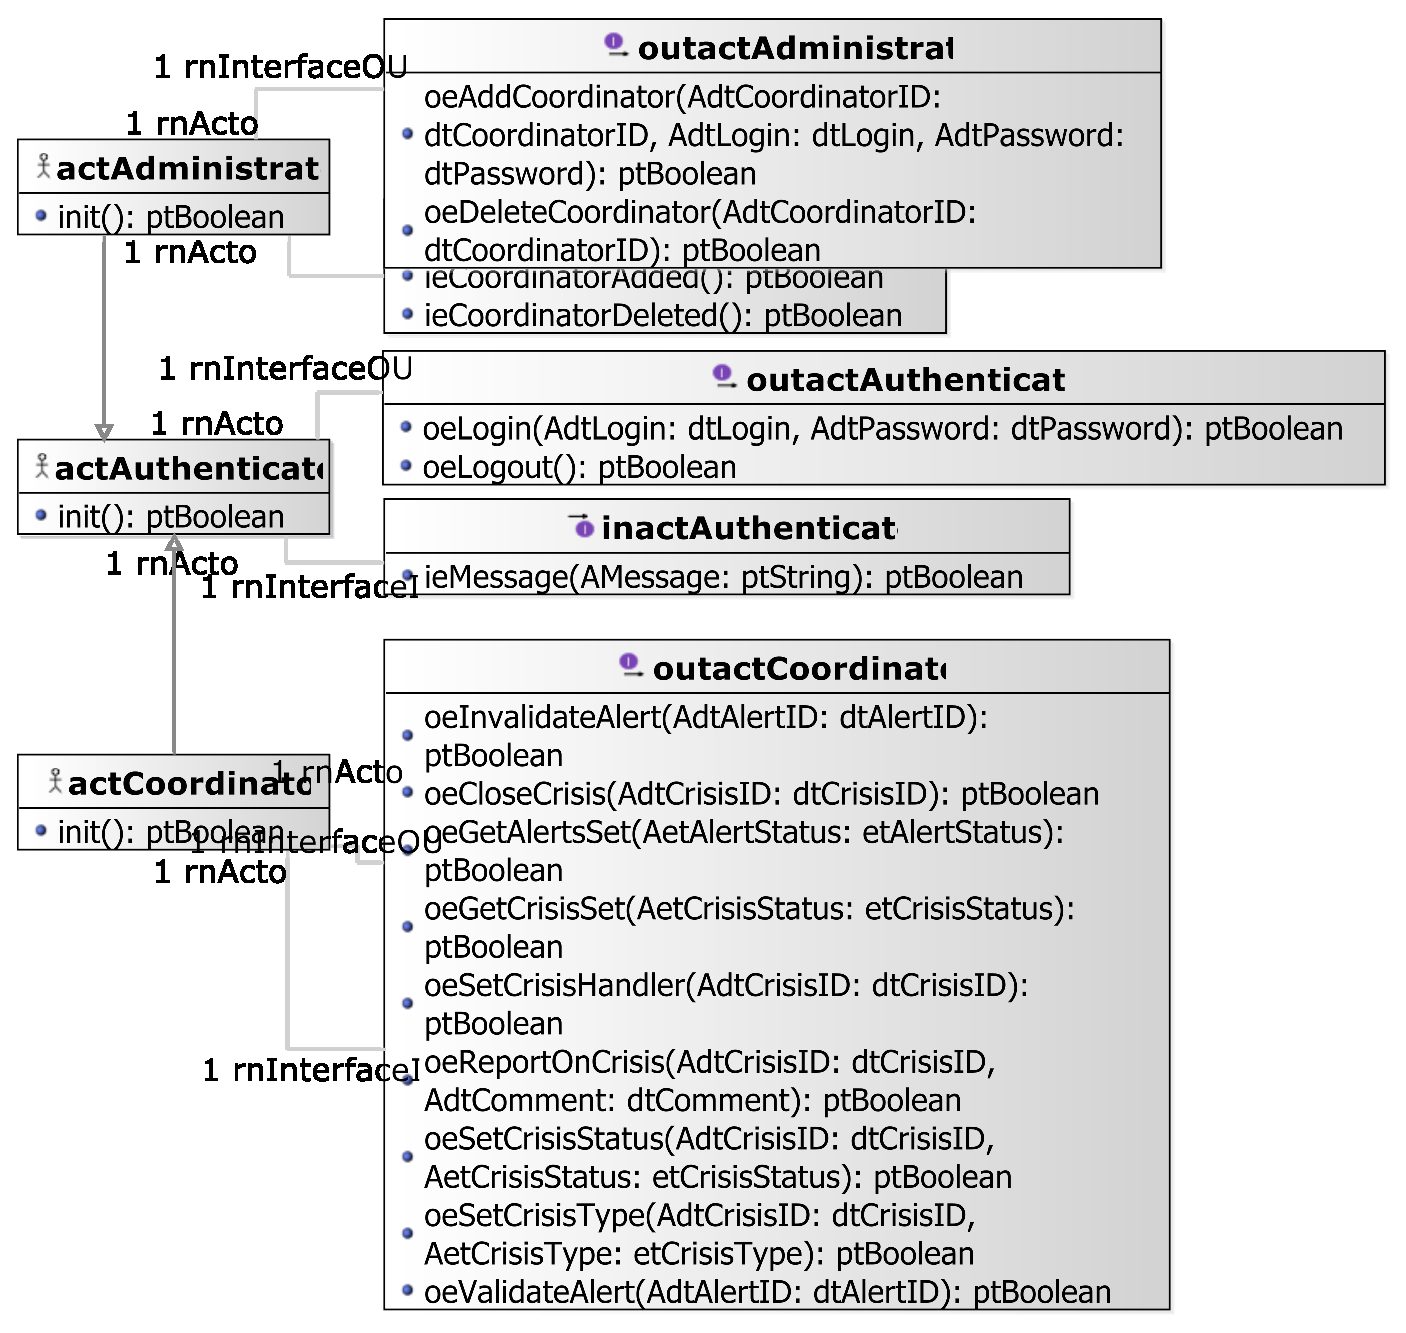
\includegraphics[
angle=0
,scale=0.80
]{./images-report-gen/environment-model/local/01/em-lv-01.eps}
\end{center}
\caption[Environment Model - Local View 01 - environment model local view - Part ]{Environment Model - Local View 01. environment model local view - Part 1.}
\label{fig:lu.uni.lassy.excalibur.examples.icrash-EM-view-local-01}
\end{figure}
\vspace{0.5cm} 

\section{Local view 02}
\label{sec:lu.uni.lassy.excalibur.examples.icrash-EM-view-02-local}

Figure \ref{fig:lu.uni.lassy.excalibur.examples.icrash-EM-view-local-02} 
shows the local view giving the second part the environment model of the system in term of its state class, actors with their input and output interfaces and all related associations.


\begin{figure}[htbp] 
\label{fig:lu.uni.lassy.excalibur.examples.icrash-EM}
\begin{center}
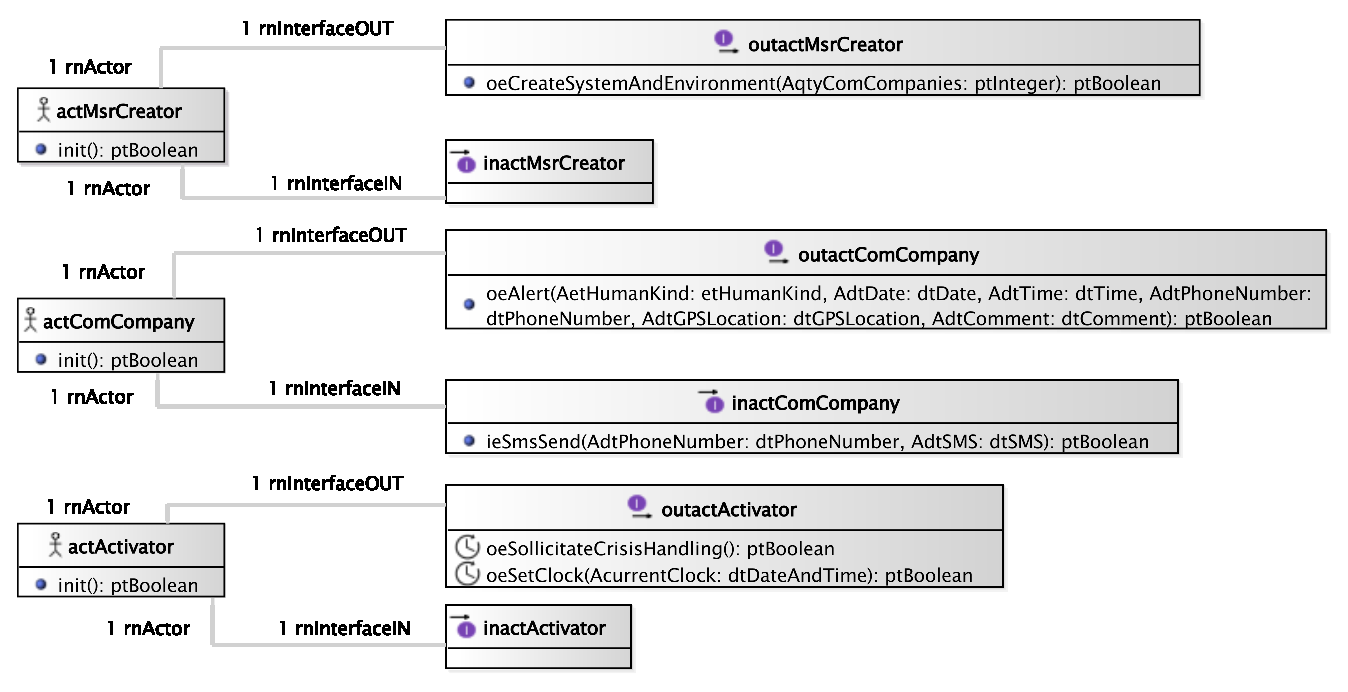
\includegraphics[
angle=0
,scale=0.80
]{./images-report-gen/environment-model/local/02/em-lv-02.eps}
\end{center}
\caption[Environment Model - Local View 02 - environment model local view - Part ]{Environment Model - Local View 02. environment model local view - Part 2.}
\label{fig:lu.uni.lassy.excalibur.examples.icrash-EM-view-local-02}
\end{figure}
\vspace{0.5cm} 

\section{Local view 03}
\label{sec:lu.uni.lassy.excalibur.examples.icrash-EM-view-03-local}

Figure \ref{fig:lu.uni.lassy.excalibur.examples.icrash-EM-view-local-03} shows the local view for the administrator actor and interfaces


\begin{figure}[htbp] 
\label{fig:lu.uni.lassy.excalibur.examples.icrash-EM}
\begin{center}
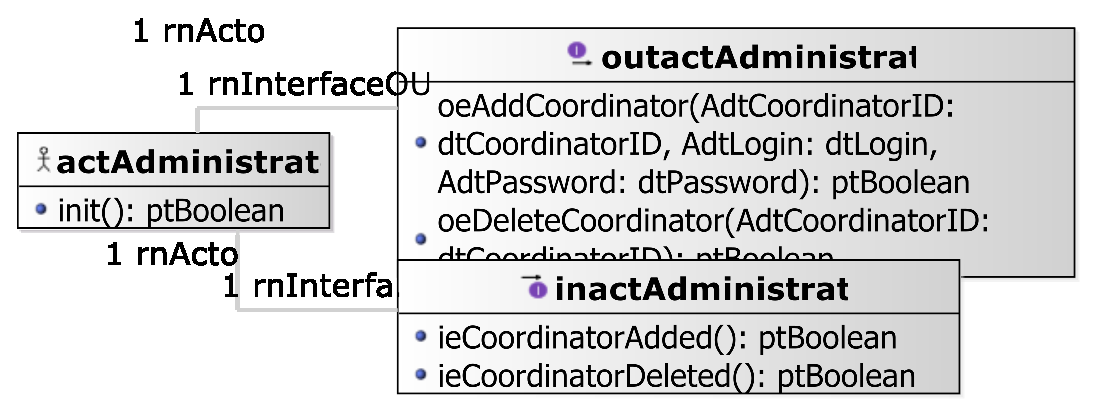
\includegraphics[
angle=0
,scale=0.80
]{./images-report-gen/environment-model/local/03/em-lv-03-parta-administrator.eps}
\end{center}
\caption[Environment Model - Local View 03 - administrator actor environment mode]{Environment Model - Local View 03. administrator actor environment model view.}
\label{fig:lu.uni.lassy.excalibur.examples.icrash-EM-view-local-03}
\end{figure}
\vspace{0.5cm} 

\section{Local view 04}
\label{sec:lu.uni.lassy.excalibur.examples.icrash-EM-view-04-local}

Figure \ref{fig:lu.uni.lassy.excalibur.examples.icrash-EM-view-local-04} shows the local view for the coordinator actor and interfaces


\begin{figure}[htbp] 
\label{fig:lu.uni.lassy.excalibur.examples.icrash-EM}
\begin{center}
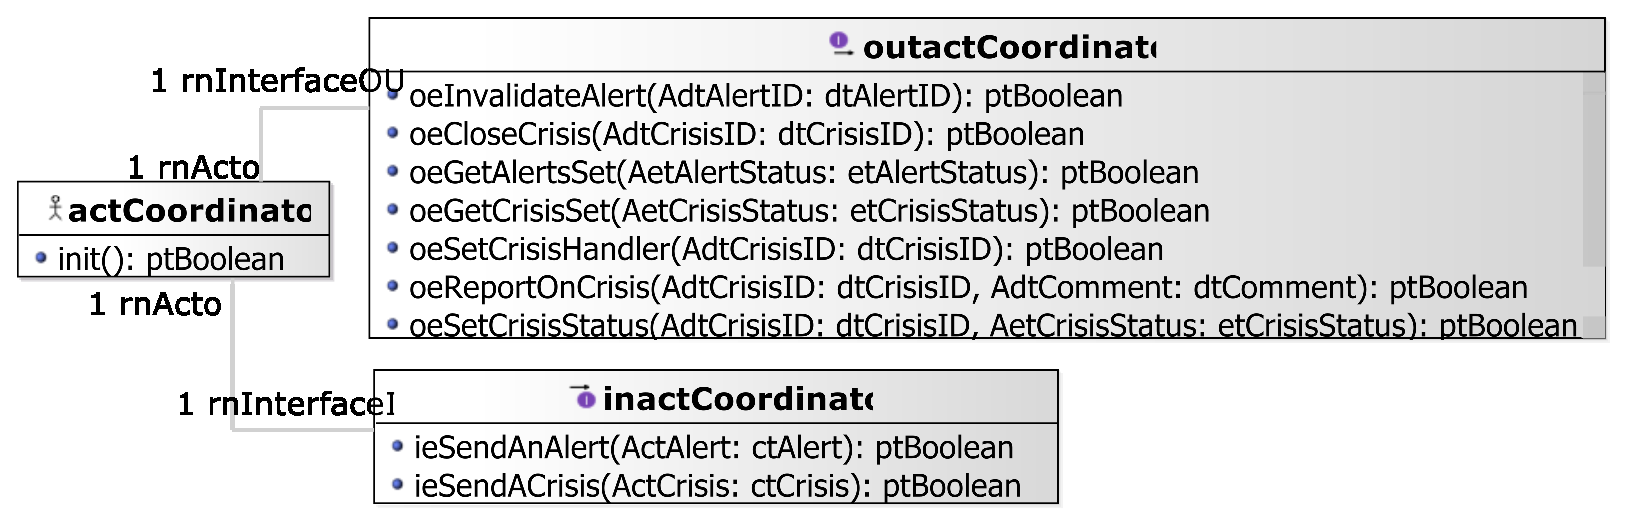
\includegraphics[
angle=0
,scale=0.80
]{./images-report-gen/environment-model/local/04/em-lv-04-partb-coordinator.eps}
\end{center}
\caption[Environment Model - Local View 04 - coordinator actor environment model ]{Environment Model - Local View 04. coordinator actor environment model view.}
\label{fig:lu.uni.lassy.excalibur.examples.icrash-EM-view-local-04}
\end{figure}
\vspace{0.5cm} 

\section{Local view 05}
\label{sec:lu.uni.lassy.excalibur.examples.icrash-EM-view-05-local}

Figure \ref{fig:lu.uni.lassy.excalibur.examples.icrash-EM-view-local-05} shows the local view for the authenticated actor and interfaces


\begin{figure}[htbp] 
\label{fig:lu.uni.lassy.excalibur.examples.icrash-EM}
\begin{center}
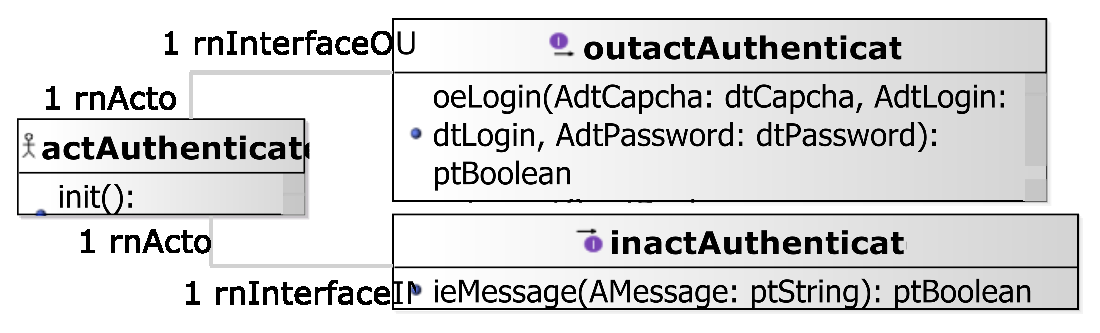
\includegraphics[
angle=0
,scale=0.80
]{./images-report-gen/environment-model/local/05/em-lv-05-partc-authenticated.eps}
\end{center}
\caption[Environment Model - Local View 05 - authenticated actor environment mode]{Environment Model - Local View 05. authenticated actor environment model local view.}
\label{fig:lu.uni.lassy.excalibur.examples.icrash-EM-view-local-05}
\end{figure}
\vspace{0.5cm} 



\section{Global view 01}
\label{sec:lu.uni.lassy.excalibur.examples.icrash-EM-view-01-global}
\clearpage

Figure \ref{fig:lu.uni.lassy.excalibur.examples.icrash-EM-view-global-01} shows a global view for all actors with their relationships with ctState


\begin{figure}[htbp] 
\label{fig:lu.uni.lassy.excalibur.examples.icrash-EM}
\begin{center}
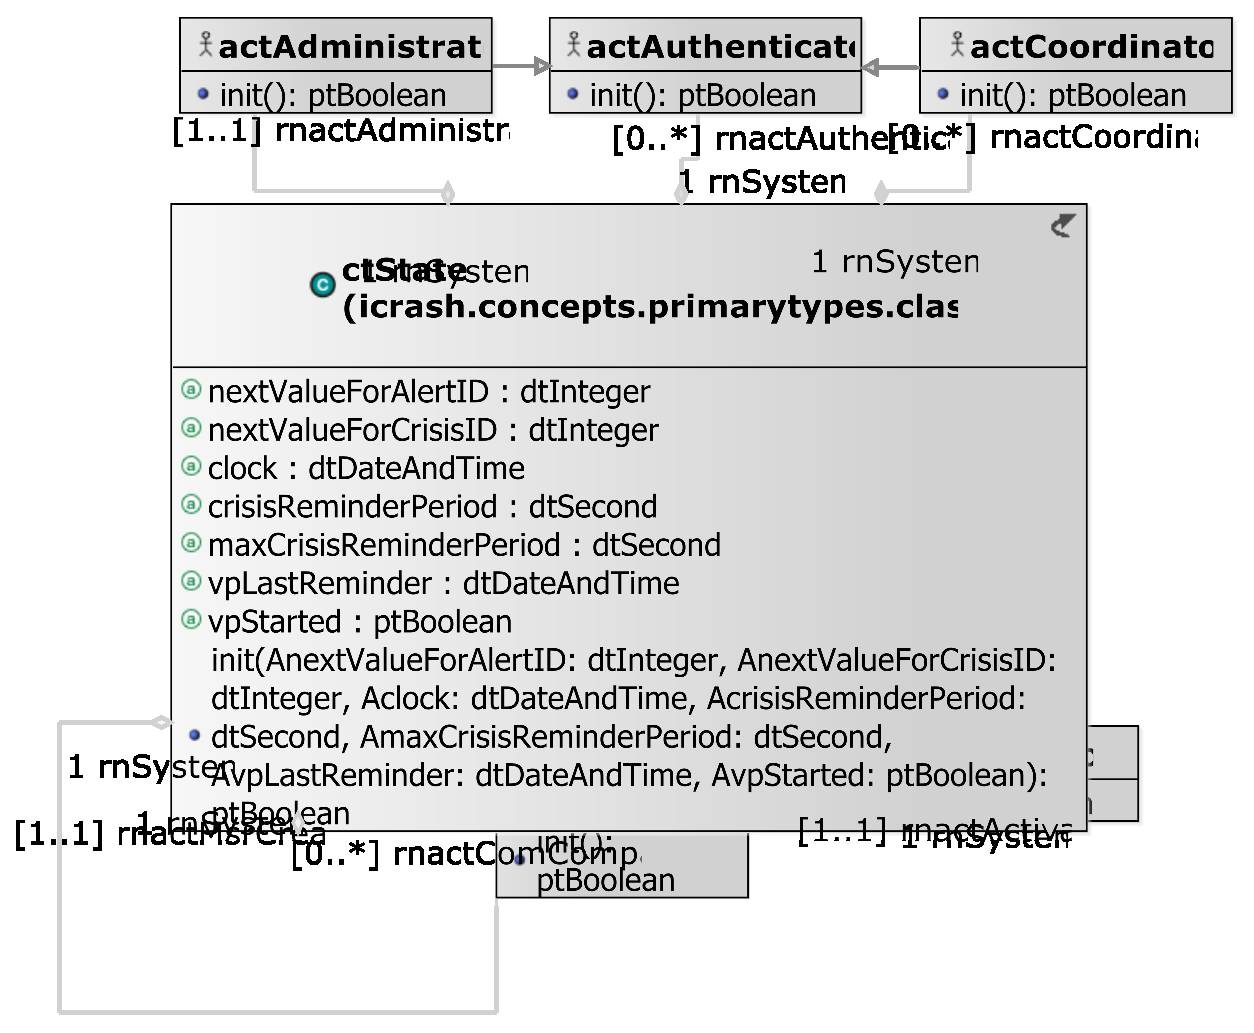
\includegraphics[
angle=0
,scale=0.80
]{./images-report-gen/environment-model/global/01/em-gv-01.eps}
\end{center}
\caption[Environment Model - Global View 01 -  em-gv-01 environment model global v]{Environment Model - Global View 01.  em-gv-01 environment model global view.}
\label{fig:lu.uni.lassy.excalibur.examples.icrash-EM-view-global-01}
\end{figure}
\vspace{0.5cm} 




\section{Actors and Interfaces Descriptions}
\label{sec:lu.uni.lassy.excalibur.examples.icrash-EM-Actors-Descriptions}


		
We provide for the given views the description of the actors together with their associated input and output interface descriptions.
\subsection{\msrcode{actActivator} Actor}


\begin{actortable}
	\addheading{Actor}
	
	\adddoublerow{actActivator}{represents a logical actor for time automatic message sending based on system's or environment status.}
	
	
	
	
	

	\addrowheading{OutputInterfaces}
	\addnumbereddoublerow{OUT}{\hypertarget{actActivator.outactActivator.oeSollicitateCrisisHandling}
			{\msrcode{[proactive] oeSollicitateCrisisHandling():ptBoolean}}}
			{used to avoid crisis to stay too long in an not handled status.}
	\addnumbereddoublerow{OUT}{\hypertarget{actActivator.outactActivator.oeSetClock}
			{\msrcode{[proactive] oeSetClock(AcurrentClock:dtDateAndTime):ptBoolean}}}
			{used to update the system's time}
	
	
\end{actortable}

\subsection{\msrcode{actAdministrator} Actor}


\begin{actortable}
	\addheading{Actor}
	
	\adddoublerow{actAdministrator}{represents an actor responsible of administration tasks for the \msricrash system.}
	
	\addrowheading{Extends}
	\addsinglerow{icrash.environment.actAuthenticated}
	
	
	
	
	\addrowheading{Operations}
	\adddoublerow{\msrcode{init():ptBoolean}}{ }
	
	

	\addrowheading{OutputInterfaces}
	\addnumbereddoublerow{OUT}{\hypertarget{actAdministrator.outactAdministrator.oeAddCoordinator}
			{\msrcode{oeAddCoordinator(AetCoordinatorType:etCoordinatorType, AdtCoordinatorID:dtCoordinatorID, AdtLogin:dtLogin, AdtPassword:dtPassword):ptBoolean}}}
			{sent to add a new coordinator in the system's post state and environment's post state.}
	\addnumbereddoublerow{OUT}{\hypertarget{actAdministrator.outactAdministrator.oeDeleteCoordinator}
			{\msrcode{oeDeleteCoordinator(AdtCoordinatorID:dtCoordinatorID):ptBoolean}}}
			{sent to delete an existing coordinator in the system's post state and environment's post state.}
	
	\addrowheading{InputInterfaces}
	\addnumbereddoublerow{IN}{\msrcode{ieCoordinatorAdded():ptBoolean}}
							 {its reception confirms the creation of the requested coodinator. }
	\addnumbereddoublerow{IN}{\msrcode{ieCoordinatorDeleted():ptBoolean}}
							 {its reception confirms the deletion of the requested coodinator. }
	
\end{actortable}

\subsection{\msrcode{actAuthenticated} Actor}


\begin{actortable}
	\addheading{Actor}
	
	\adddoublerow{actAuthenticated}{abstract actor providing reusable input and output interfaces for actors that need to authenticate themselves.}
	
	
	
	
	

	\addrowheading{OutputInterfaces}
	\addnumbereddoublerow{OUT}{\hypertarget{actAuthenticated.outactAuthenticated.oeLogin}
			{\msrcode{oeLogin(AdtCapcha:dtCapcha, AdtLogin:dtLogin, AdtPassword:dtPassword):ptBoolean}}}
			{sent to request authorization to request access secured system operations.}
	\addnumbereddoublerow{OUT}{\hypertarget{actAuthenticated.outactAuthenticated.oeLogout}
			{\msrcode{oeLogout():ptBoolean}}}
			{sent to end the secured access to specific system operations.}
	
	\addrowheading{InputInterfaces}
	\addnumbereddoublerow{IN}{\msrcode{ieMessage(AMessage:ptString):ptBoolean}}
							 {allows for receiving general textual messages.}
	
\end{actortable}

\subsection{\msrcode{actComCompany} Actor}


\begin{actortable}
	\addheading{Actor}
	
	\adddoublerow{actComCompany}{represents the communication company stakeholder ensuring the input/ouput of textual messages with humans having communicaiton devices.}
	
	
	
	
	\addrowheading{Operations}
	\adddoublerow{\msrcode{init():ptBoolean}}{ }
	
	

	\addrowheading{OutputInterfaces}
	\addnumbereddoublerow{OUT}{\hypertarget{actComCompany.outactComCompany.oeAlert}
			{\msrcode{oeAlert(AetHumanKind:etHumanKind, AdtDate:dtDate, AdtTime:dtTime, AdtPhoneNumber:dtPhoneNumber, AdtGPSLocation:dtGPSLocation, AdtComment:dtComment):ptBoolean}}}
			{sent to alert of a potential crisis situation.}
	
	\addrowheading{InputInterfaces}
	\addnumbereddoublerow{IN}{\msrcode{ieSmsSend(AdtPhoneNumber:dtPhoneNumber, AdtSMS:dtSMS):ptBoolean}}
							 {allows for receiving textual messages to be dispatched to the communication company customers having the provided phone number.}
	
\end{actortable}

\subsection{\msrcode{actCoordinator} Actor}


\begin{actortable}
	\addheading{Actor}
	
	\adddoublerow{actCoordinator}{represents actor responsible of handling one or several crisis for the \msricrash system.}
	
	\addrowheading{Extends}
	\addsinglerow{icrash.environment.actAuthenticated}
	
	
	
	
	\addrowheading{Operations}
	\adddoublerow{\msrcode{init():ptBoolean}}{ }
	
	

	\addrowheading{OutputInterfaces}
	\addnumbereddoublerow{OUT}{\hypertarget{actCoordinator.outactCoordinator.oeInvalidateAlert}
			{\msrcode{oeInvalidateAlert(AdtAlertID:dtAlertID):ptBoolean}}}
			{sent to indicate that an alert should be considered as closed.}
	\addnumbereddoublerow{OUT}{\hypertarget{actCoordinator.outactCoordinator.oeCloseCrisis}
			{\msrcode{oeCloseCrisis(AdtCrisisID:dtCrisisID):ptBoolean}}}
			{sent to indicate that a crisis should be considered as closed.}
	\addnumbereddoublerow{OUT}{\hypertarget{actCoordinator.outactCoordinator.oeGetAlertsSet}
			{\msrcode{oeGetAlertsSet(AetAlertStatus:etAlertStatus):ptBoolean}}}
			{sent to request all the ctAlert instances having a specific status.}
	\addnumbereddoublerow{OUT}{\hypertarget{actCoordinator.outactCoordinator.oeGetCrisisSet}
			{\msrcode{oeGetCrisisSet(AetCrisisStatus:etCrisisStatus):ptBoolean}}}
			{sent to request all the ctCrisis instances having a specific status.}
	\addnumbereddoublerow{OUT}{\hypertarget{actCoordinator.outactCoordinator.oeSetCrisisHandler}
			{\msrcode{oeSetCrisisHandler(AdtCrisisID:dtCrisisID):ptBoolean}}}
			{sent to declare himself as been the handler of a crisis having the specified id.}
	\addnumbereddoublerow{OUT}{\hypertarget{actCoordinator.outactCoordinator.oeReportOnCrisis}
			{\msrcode{oeReportOnCrisis(AdtCrisisID:dtCrisisID, AdtComment:dtComment):ptBoolean}}}
			{sent to update the textual information available for a specific handled crisis.}
	\addnumbereddoublerow{OUT}{\hypertarget{actCoordinator.outactCoordinator.oeSetCrisisStatus}
			{\msrcode{oeSetCrisisStatus(AdtCrisisID:dtCrisisID, AetCrisisStatus:etCrisisStatus):ptBoolean}}}
			{sent to define the handling status of a specific crisis.}
	\addnumbereddoublerow{OUT}{\hypertarget{actCoordinator.outactCoordinator.oeSetCrisisType}
			{\msrcode{oeSetCrisisType(AdtCrisisID:dtCrisisID, AetCrisisType:etCrisisType):ptBoolean}}}
			{sent to define the gravity type of a specific crisis.}
	\addnumbereddoublerow{OUT}{\hypertarget{actCoordinator.outactCoordinator.oeValidateAlert}
			{\msrcode{oeValidateAlert(AdtAlertID:dtAlertID):ptBoolean}}}
			{sent to indicate that a specific alert is not a fake.}
	
	\addrowheading{InputInterfaces}
	\addnumbereddoublerow{IN}{\msrcode{ieSendAnAlert(ActAlert:ctAlert):ptBoolean}}
							 {allows for receiving a requested ctAlert instance.}
	\addnumbereddoublerow{IN}{\msrcode{ieSendACrisis(ActCrisis:ctCrisis):ptBoolean}}
							 {allows for receiving a requested ctCrisis instance.}
	
\end{actortable}

\subsection{\msrcode{actHospital} Actor}


\begin{actortable}
	\addheading{Actor}
	
	\adddoublerow{actHospital}{Represents actor that is responsible for handling those crisises, that are connected to medical injuries.}
	
	\addrowheading{Extends}
	\addsinglerow{icrash.environment.actAuthenticated}
	
	
	
	
	\addrowheading{Operations}
	\adddoublerow{\msrcode{init():ptBoolean}}{}
	
	

	\addrowheading{OutputInterfaces}
	\addnumbereddoublerow{OUT}{\hypertarget{actHospital.outactHospital.oeCloseCrisis}
			{\msrcode{oeCloseCrisis(AdtCrisisID:dtCrisisID):ptBoolean}}}
			{sent to indicate that a crisis should be considered as closed.}
	\addnumbereddoublerow{OUT}{\hypertarget{actHospital.outactHospital.oeGetCrisisSet}
			{\msrcode{oeGetCrisisSet(AetCrisisStatus:etCrisisStatus):ptBoolean}}}
			{sent to request all the ctCrisis instances having a specific status.}
	\addnumbereddoublerow{OUT}{\hypertarget{actHospital.outactHospital.oeSetCrisisHandler}
			{\msrcode{oeSetCrisisHandler(AdtCrisisID:dtCrisisID):ptBoolean}}}
			{sent to declare himself as been the handler of a crisis having the specified id.}
	\addnumbereddoublerow{OUT}{\hypertarget{actHospital.outactHospital.oeSetCrisisStatus}
			{\msrcode{oeSetCrisisStatus(AdtCrisisID:dtCrisisID, AetCrisisStatus:etCrisisStatus):ptBoolean}}}
			{sent to define the handling status of a specific crisis.}
	\addnumbereddoublerow{OUT}{\hypertarget{actHospital.outactHospital.oeSetCrisisType}
			{\msrcode{oeSetCrisisType(AdtCrisisID:dtCrisisID, AetCrisisType:etCrisisType):ptBoolean}}}
			{sent to define the gravity type of a specific crisis.}
	
	\addrowheading{InputInterfaces}
	\addnumbereddoublerow{IN}{\msrcode{ieSendACrisis(ActCrisis:ctCrisis):ptBoolean}}
							 {allows for receiving a requested ctCrisis instance.}
	
\end{actortable}

\subsection{\msrcode{actMsrCreator} Actor}


\begin{actortable}
	\addheading{Actor}
	
	\adddoublerow{actMsrCreator}{Represents the creator stakeholder in charge of state and environment initialization.}
	
	
	
	
	\addrowheading{Operations}
	\adddoublerow{\msrcode{init():ptBoolean}}{ }
	
	

	\addrowheading{OutputInterfaces}
	\addnumbereddoublerow{OUT}{\hypertarget{actMsrCreator.outactMsrCreator.oeCreateSystemAndEnvironment}
			{\msrcode{oeCreateSystemAndEnvironment(AqtyComCompanies:ptInteger):ptBoolean}}}
			{sent to request the initialization of the system's class instances and the environment actors instances.}
	
	
\end{actortable}

